\section{Graphs in Waiting}
\begin{figure}[t]
    \centering
    \caption{Distribution of Racial Imagery of Police Departments Surveyed in LEMAS 2016} 
	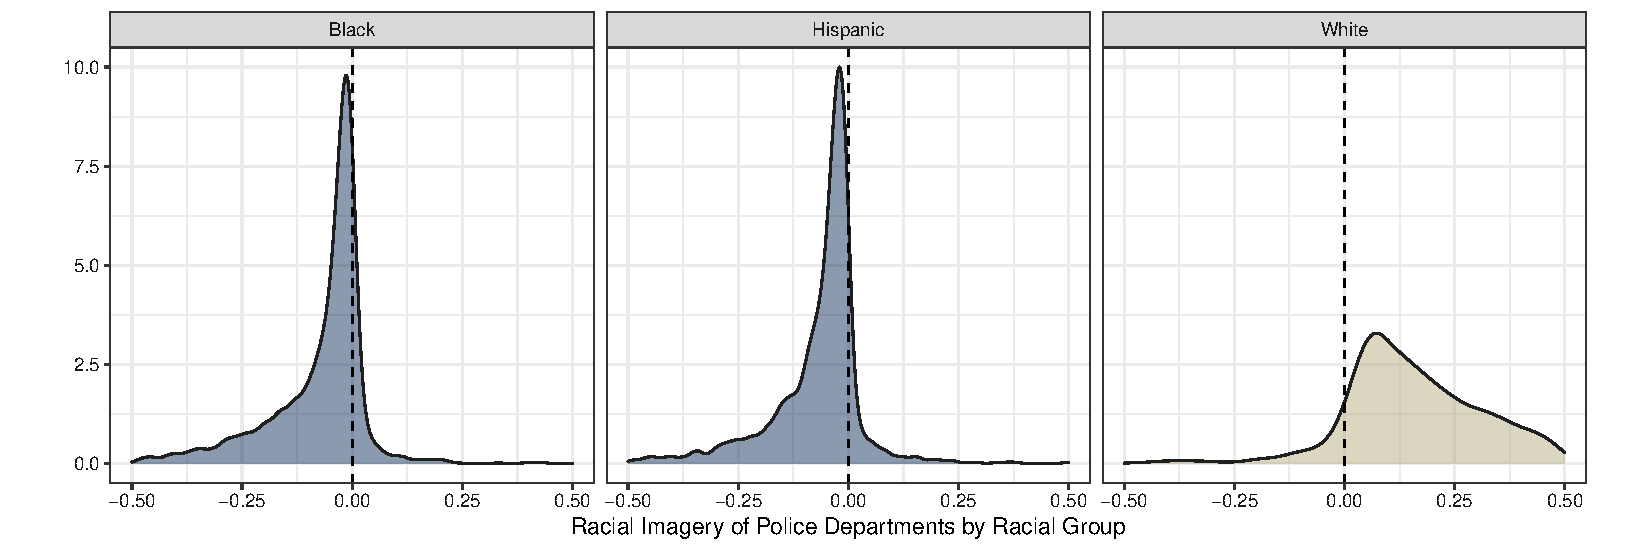
\includegraphics[width = \linewidth]{figures/desc-lemas2.pdf}
    \label{fig:lemas-density}
    \fnote{On the horizontal axis, a positive value indicates that the corresponding racial group is excessively represented in local police departments, and a negative value the otherwise.}
\end{figure}

\begin{figure}[t]  \centering
    \caption{Geographic Coverage of LEMAS 2016 at the County Level} 
	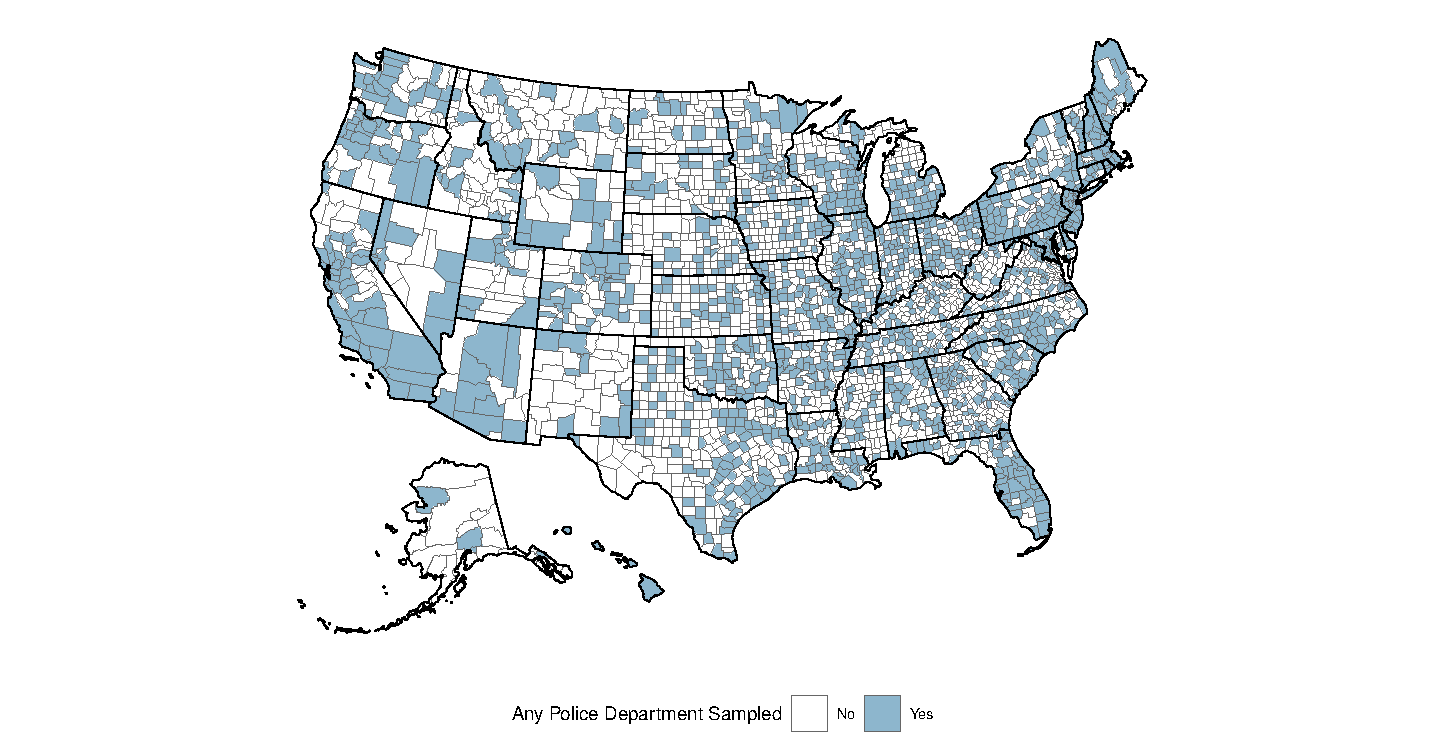
\includegraphics[width = \linewidth]{figures/lemas-map-ct.pdf}
    \label{fig:lemas-geo}
    \fnote{Counties are colored blue where at least one police department within its jurisdiction is surveyed in LEMAS 2016.}
\end{figure}

\begin{figure}[t]  \centering
    \caption{Racial Imagery of Police and White Attitudes toward Policing} 
	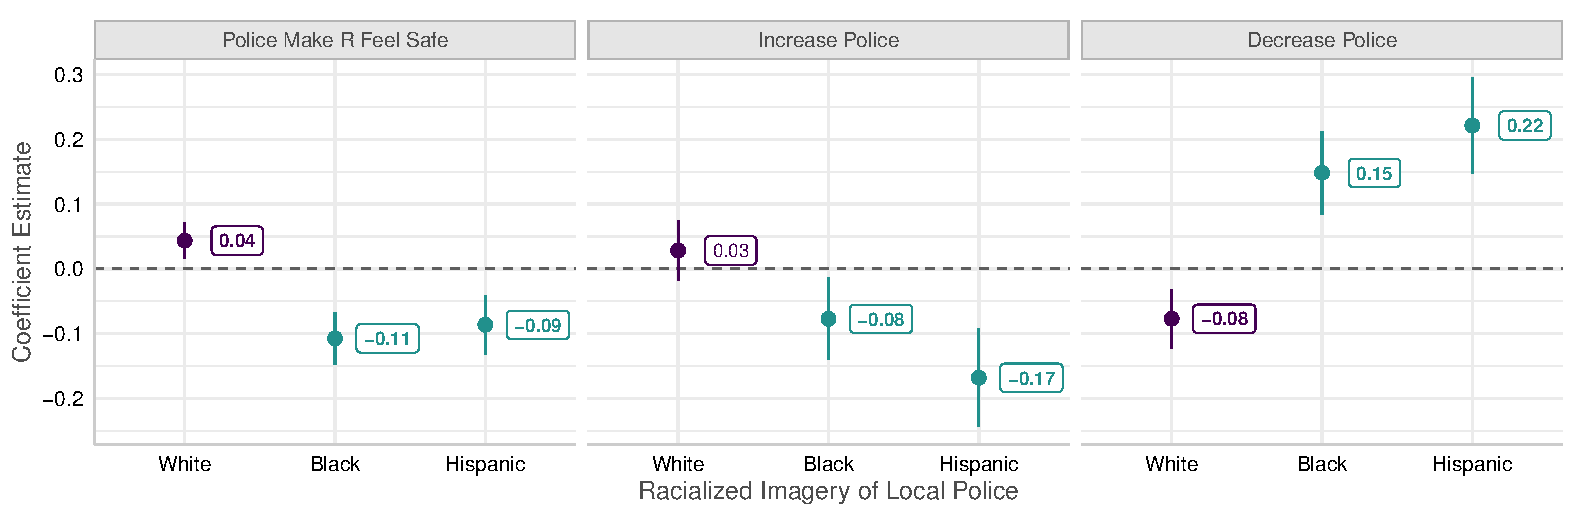
\includegraphics[width = \linewidth]{figures/imagery & attitudes 2}
    \label{fig:baseline}
    \fnote{}
\end{figure}

\begin{figure}[t]  \centering
    \caption{Racial Divides on Policing Moderated by Racial Imagery of Police}
	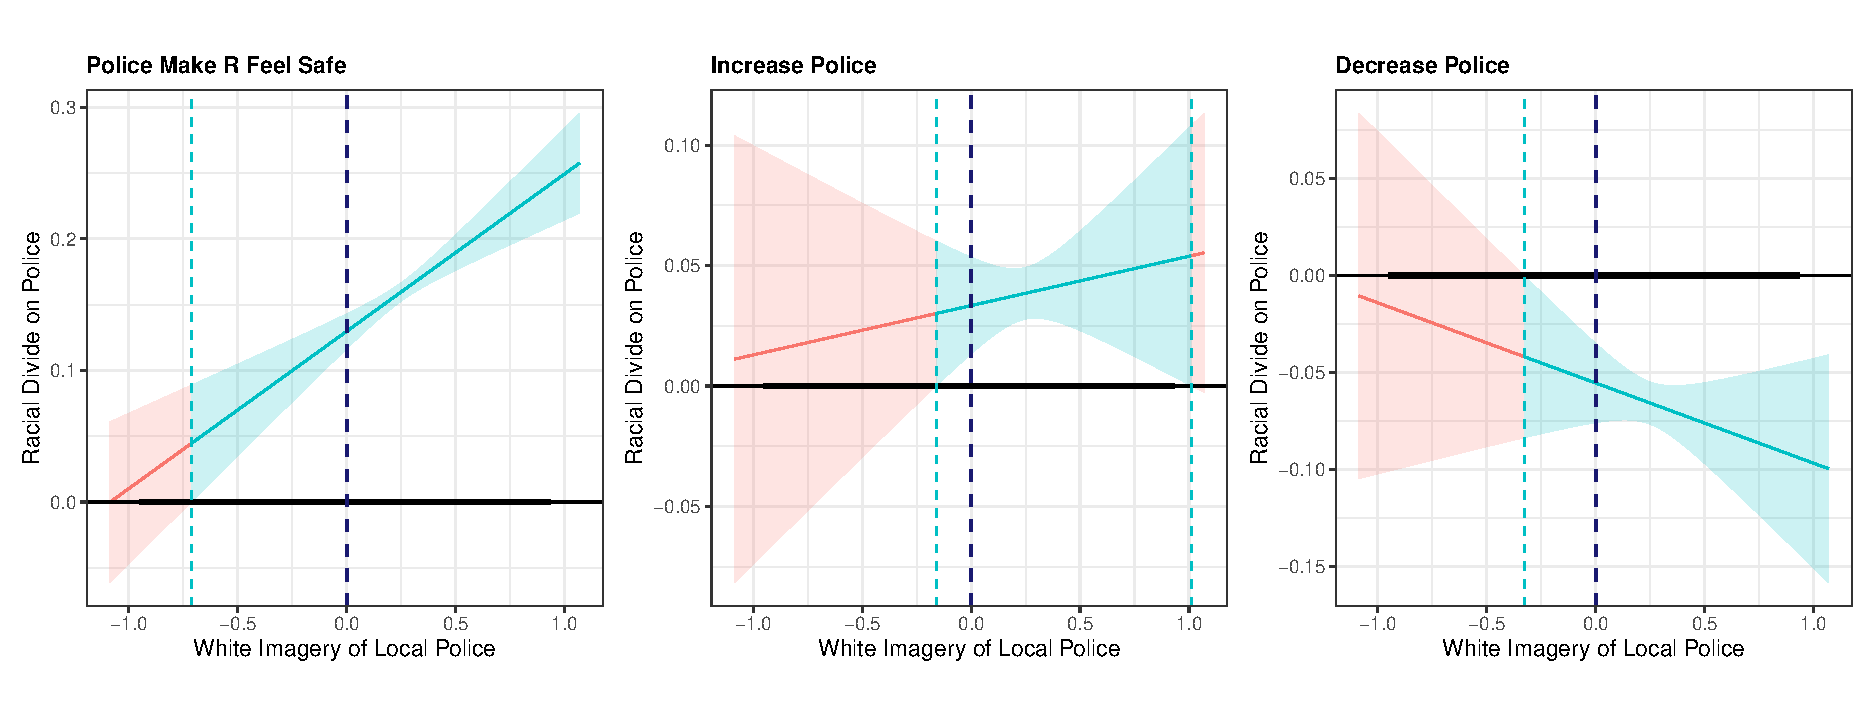
\includegraphics[width = \linewidth]{figures/divide moderation}
    \label{fig:divides}
    \fnote{}
\end{figure}

\begin{figure}[t]  \centering
    \caption{Racial Imagery Moderates Whites' Attitudinal Reaction to Police Violence}
	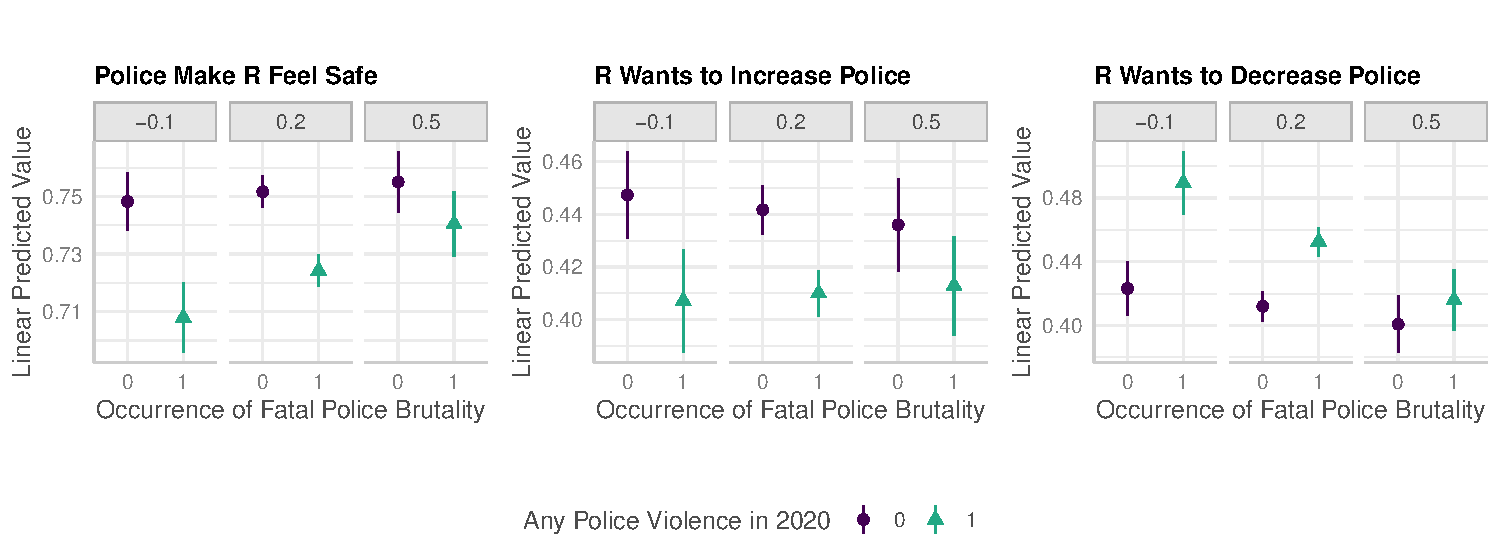
\includegraphics[width = \linewidth]{figures/reaction moderation}
    \label{fig:moderation}
    \fnote{}
\end{figure}

\begin{figure}[t]  \centering
    \caption{Moderation Effect of Racial Imagery Contingent upon Racial Groups Victimized by Police Violence}
	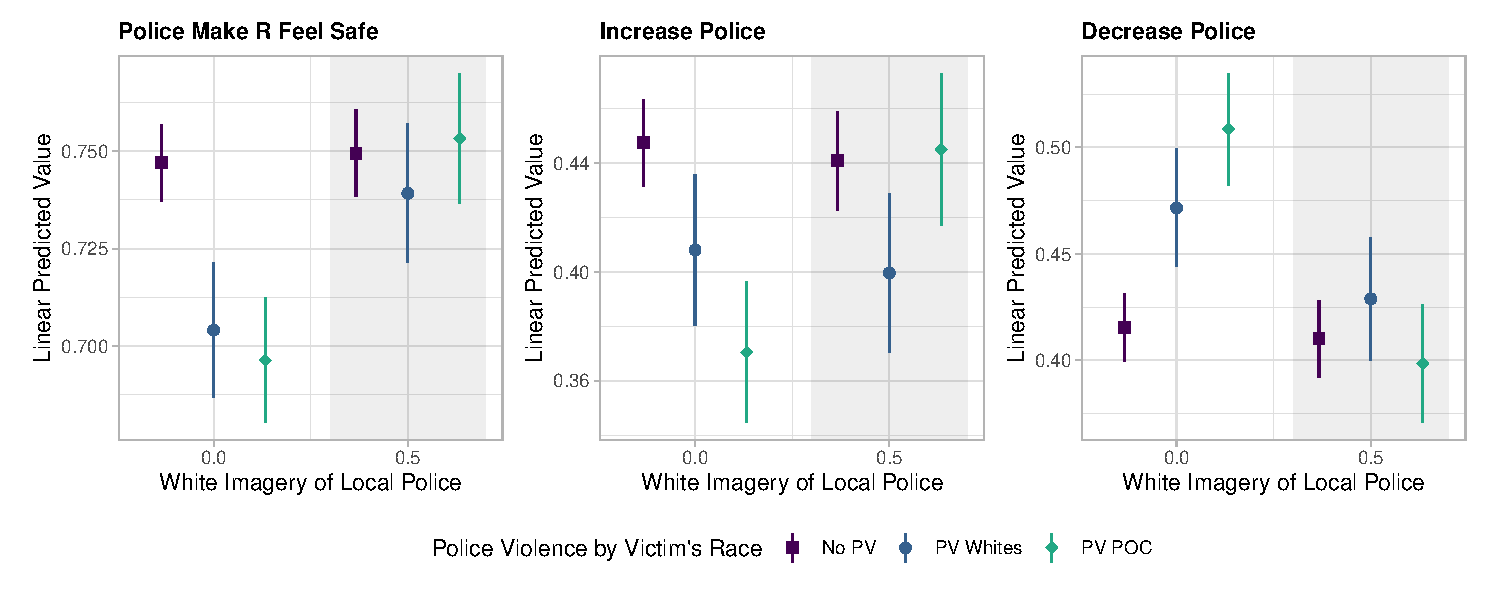
\includegraphics[width = \linewidth]{figures/racial component}
    \label{fig:racial component}
    \fnote{}
\end{figure}


\begin{table}

\caption{Racial Imagery of Local Police Affects Racial Divide on Policing.}
\centering
\begin{tabular}[t]{lccc}
\toprule
  & Police Felt as Safe & Increase Police & Decrease Police\\
\midrule
Racial Divide & 0.221*** & 0.048** & -0.072***\\
 & (0.016) & (0.016) & (0.016)\\
White Imagery of Police & -0.168*** & 0.003 & 0.018\\
 & (0.049) & (0.048) & (0.048)\\
Racial Divide × White Imagery & 0.182** & 0.019 & -0.039\\
 & (0.055) & (0.057) & (0.055)\\
\midrule
Num.Obs. & 39551 & 39597 & 39589\\
R2 & 0.076 & 0.002 & 0.007\\
\bottomrule
\multicolumn{4}{l}{\rule{0pt}{1em}This is the note of your regression table.}\\
\multicolumn{4}{l}{\rule{0pt}{1em}+ p $<$ 0.1, * p $<$ 0.05, ** p $<$ 0.01, *** p $<$ 0.001}\\
\end{tabular}
\end{table}


\begin{table}

\caption{Racial Imagery of Local Police Moderates Attitudinal Reaction to Police Violence.}
\centering
\begin{tabular}[t]{lccc}
\toprule
  & Police Felt as Safe & Increase Police & Decrease Police\\
\midrule
White Imagery of Police & \num{0.006} & \num{-0.009} & \num{-0.014}\\
 & (\num{0.018}) & (\num{0.029}) & (\num{0.029})\\
Any Police Violence in 2020 & \num{-0.047}*** & \num{-0.057}*** & \num{0.074}***\\
 & (\num{0.008}) & (\num{0.013}) & (\num{0.013})\\
Police Violence × White Imagery & \num{0.087}** & \num{0.078}+ & \num{-0.142}**\\
 & (\num{0.028}) & (\num{0.045}) & (\num{0.045})\\
\midrule
Num.Obs. & \num{26016} & \num{26039} & \num{26036}\\
R2 & \num{0.004} & \num{0.002} & \num{0.003}\\
\bottomrule
\multicolumn{4}{l}{\rule{0pt}{1em}This is the note of your regression table.}\\
\multicolumn{4}{l}{\rule{0pt}{1em}+ p $<$ 0.1, * p $<$ 0.05, ** p $<$ 0.01, *** p $<$ 0.001}\\
\end{tabular}
\end{table}


\begin{table}

\caption{Moderating Effect of Racial Imagery Depends upon Racial Groups Victimized by Police Violence}
\centering
\begin{tabular}[t]{lccc}
\toprule
  & Police Felt as Safe & Increase Police & Decrease Police\\
\midrule
White Imagery of Police & 0.007 & -0.013 & -0.010\\
 & (0.027) & (0.029) & (0.029)\\
PV Whites & -0.065*** & -0.039* & 0.056***\\
 & (0.015) & (0.016) & \vphantom{1} (0.016)\\
PV POC & -0.076*** & -0.077*** & 0.093***\\
 & (0.015) & (0.016) & (0.016)\\
White Imagery × PV Whites & 0.098+ & -0.003 & -0.075\\
 & (0.053) & (0.057) & (0.057)\\
White Imagery × PV POC & 0.164** & 0.162** & -0.210***\\
 & (0.053) & (0.058) & (0.058)\\
\midrule
Num.Obs. & 26016 & 26039 & 26036\\
R2 & 0.004 & 0.002 & 0.003\\
\bottomrule
\multicolumn{4}{l}{\rule{0pt}{1em}This is the note of your regression table.}\\
\multicolumn{4}{l}{\rule{0pt}{1em}+ p $<$ 0.1, * p $<$ 0.05, ** p $<$ 0.01, *** p $<$ 0.001}\\
\end{tabular}
\end{table}



